%%%%%%%%%%%%%%%%%%%%%%%%%%%%%%%%%%%%%%%%%%%%%%%%%%%%%%%%%%%%%%%%%%%%%%%%%%%%%%%%
%% MASTER'S THESIS — Pratik Khadka
%% Single-file version for Overleaf
%% Upload this file + references.bib to Overleaf and compile with pdfLaTeX
%% Compile order: pdflatex → bibtex → pdflatex → pdflatex
%%%%%%%%%%%%%%%%%%%%%%%%%%%%%%%%%%%%%%%%%%%%%%%%%%%%%%%%%%%%%%%%%%%%%%%%%%%%%%%%

\documentclass[12pt, a4paper, twoside, openright]{report}

% ── Packages ────────────────────────────────────────────────────────────────
\usepackage[utf8]{inputenc}
\usepackage[T1]{fontenc}
\usepackage{lmodern}
\usepackage{microtype}
\usepackage[english]{babel}
\usepackage[left=3cm,right=2.5cm,top=2.5cm,bottom=2.5cm,bindingoffset=0.5cm]{geometry}
\usepackage{setspace}\onehalfspacing
\usepackage{fancyhdr}
\pagestyle{fancy}\fancyhf{}
\fancyhead[LE]{\leftmark}\fancyhead[RO]{\rightmark}\fancyfoot[C]{\thepage}
\renewcommand{\headrulewidth}{0.4pt}
\usepackage{amsmath,amssymb}
\usepackage{graphicx}\graphicspath{{thesis_figures/}{figures/}}
\usepackage{float}
\usepackage{subcaption}
\usepackage{booktabs,tabularx,multirow,array}
\usepackage[dvipsnames]{xcolor}
\usepackage{listings}
\lstset{basicstyle=\ttfamily\small,keywordstyle=\color{blue}\bfseries,
  commentstyle=\color{gray}\itshape,stringstyle=\color{red},
  numbers=left,numberstyle=\tiny\color{gray},numbersep=8pt,
  frame=single,breaklines=true,captionpos=b,tabsize=2}
\usepackage[ruled,vlined,linesnumbered]{algorithm2e}
\usepackage[colorlinks=true,linkcolor=NavyBlue,citecolor=ForestGreen,
  urlcolor=BrickRed,bookmarks=true,bookmarksnumbered=true]{hyperref}
\usepackage[numbers,sort&compress]{natbib}
\usepackage[acronym,toc,nonumberlist]{glossaries}
\usepackage{siunitx}\sisetup{per-mode=symbol}
\usepackage[toc,page]{appendix}
\usepackage{caption}
\captionsetup[table]{position=bottom,skip=6pt}
\captionsetup[figure]{position=bottom,skip=6pt}

% ── Acronyms ────────────────────────────────────────────────────────────────
\makeglossaries
\newacronym{fl}{FL}{Federated Learning}
\newacronym{tinyml}{TinyML}{Tiny Machine Learning}
\newacronym{lorawan}{LoRaWAN}{Long Range Wide Area Network}
\newacronym{ttn}{TTN}{The Things Network}
\newacronym{fedavg}{FedAvg}{Federated Averaging}
\newacronym{pdr}{PDR}{Packet Delivery Ratio}
\newacronym{rssi}{RSSI}{Received Signal Strength Indicator}
\newacronym{snr}{SNR}{Signal-to-Noise Ratio}
\newacronym{sf}{SF}{Spreading Factor}
\newacronym{adr}{ADR}{Adaptive Data Rate}
\newacronym{mcu}{MCU}{Microcontroller Unit}
\newacronym{tflite}{TFLite}{TensorFlow Lite}
\newacronym{iid}{IID}{Independent and Identically Distributed}
\newacronym{rmse}{RMSE}{Root Mean Square Error}
\newacronym{mae}{MAE}{Mean Absolute Error}
\newacronym{iot}{IoT}{Internet of Things}
\newacronym{lpwan}{LPWAN}{Low Power Wide Area Network}
\newacronym{sram}{SRAM}{Static Random Access Memory}
\newacronym{otaa}{OTAA}{Over-The-Air Activation}

% ── Metadata ────────────────────────────────────────────────────────────────
\newcommand{\thesistitle}{Decentralized Edge Intelligence for LoRaWAN: Federated Learning for Environment-Driven Path Loss and Link Quality Modeling}
\newcommand{\authorname}{Pratik Khadka}
\newcommand{\supervisorname}{Prof.\ Dr.\ Kristof Van Laerhoven}
\newcommand{\secondexaminer}{M.Sc.\ Nahshon Mokua Obiri}
\newcommand{\universityname}{University of Siegen}
\newcommand{\departmentname}{Department of Electrical Engineering and Computer Science}
\newcommand{\programmename}{Ubiquitous Computing}
\newcommand{\matrikelnr}{1833319}
\newcommand{\submissiondate}{15.\ June 2026}

%%%%%%%%%%%%%%%%%%%%%%%%%%%%%%%%%%%%%%%%%%%%%%%%%%%%%%%%%%%%%%%%%%%%%%%%%%%%%%%%
\begin{document}
\pagenumbering{Roman}

% ══════════════════════════════════════════════════════════════════════════════
% TITLE PAGE
% ══════════════════════════════════════════════════════════════════════════════
\begin{titlepage}
  \noindent
  
\includegraphics[height=1.5cm]{UNiversity siegen.png}\hfill
  
\includegraphics[height=1.2cm]{eminent.png}\hfill
  
\includegraphics[height=1.5cm]{ubiquitous Computing.png}

  \vspace{3cm}
  \centering

  {\large\textsc{\universityname}}\\[1.5cm]

  {\LARGE\bfseries \thesistitle}\\[2cm]

  {\Large\textsc{Master's Thesis}}\\[0.3cm]
  {\large\textit{\programmename}}\\[1.5cm]

  {\Large\textit{\authorname}}\\[0.3cm]
  {\normalsize Matriculation number: \matrikelnr}\\[1.5cm]

  {\normalsize \submissiondate}

  \vfill

  \begin{flushleft}
    \textbf{Examiner}\\[0.3cm]
    \begin{tabular}{@{}l@{\hspace{4cm}}l@{}}
      Prof.\ Dr.\ Kristof \textsc{Van Laerhoven} & \universityname \\
      M.Sc.\ Nahshon Mokua \textsc{Obiri}        & \universityname \\
    \end{tabular}
  \end{flushleft}
\end{titlepage}


% ══════════════════════════════════════════════════════════════════════════════
% PAGE 2: BLANK PAGE
% ══════════════════════════════════════════════════════════════════════════════
\newpage
\thispagestyle{empty}
\mbox{}
\newpage

% ══════════════════════════════════════════════════════════════════════════════
% PAGE 3: SUBMISSION DETAILS
% ══════════════════════════════════════════════════════════════════════════════
\thispagestyle{empty}
\noindent This Master's Thesis was submitted in accordance with the regulations of the University of Siegen for the degree of Master of Science (M.\,Sc.) according to the examination regulations FPO 2021.

\vfill
\begin{flushleft}
\textbf{Examiner}\\[0.3cm]
Prof.\ Dr.\ Kristof \textsc{Van Laerhoven}\\
M.Sc.\ Nahshon Mokua \textsc{Obiri}
\end{flushleft}
\newpage

% ══════════════════════════════════════════════════════════════════════════════
% PAGE 4: BLANK PAGE
% ══════════════════════════════════════════════════════════════════════════════
\thispagestyle{empty}
\mbox{}
\newpage

% ══════════════════════════════════════════════════════════════════════════════
% PAGE 5: DECLARATION OF ORIGINALITY
% ══════════════════════════════════════════════════════════════════════════════
\chapter*{Declaration of Originality}
\vspace*{-1cm}
\addcontentsline{toc}{chapter}{Declaration of Originality}
I affirm that I have written my thesis independently and that I have not used any sources or aids other than those indicated, and that I have clearly indicated citations.

All passages that are taken from other works in terms of wording or meaning (including translations) have been clearly marked as borrowed in each individual case, with precise indication of the source (including the World Wide Web and other electronic data collections). This also applies to attached drawings, pictorial representations, sketches and the like. I take note that the proven omission of the indication of origin will be considered as attempted deception.

\vspace{3cm}
\noindent
\begin{tabular}{@{}p{6cm}@{\hspace{1.5cm}}p{6cm}@{}}
  \dotfill & \dotfill \\
  \centering Location, Date & \centering Signature \arraybackslash
\end{tabular}
\newpage

% ══════════════════════════════════════════════════════════════════════════════
% PAGE 6: BLANK PAGE
% ══════════════════════════════════════════════════════════════════════════════
\thispagestyle{empty}
\mbox{}
\newpage

% ══════════════════════════════════════════════════════════════════════════════
% ABSTRACT
% ══════════════════════════════════════════════════════════════════════════════

\chapter*{Abstract}
\addcontentsline{toc}{chapter}{Abstract}

Wireless signal attenuation in indoor Long Range Wide Area Networks (\gls{lorawan}) is governed by both structural building configurations and dynamic microclimatic fluctuations, limiting the predictive reliability of standard distance-only path loss models. While integrating localized environmental covariates (such as temperature, relative humidity, carbon dioxide, barometric pressure, and PM2.5 particulate matter) into regression frameworks improves path loss estimation, existing centralized approaches necessitate the continuous uploading of raw sensor streams. This constant transmission creates severe channel congestion, threatens compliance with strict LPWAN duty-cycle regulations, and presents critical data privacy risks.

This thesis addresses these challenges by introducing a decentralized, communication-compliant \gls{fl} framework combined with on-device \gls{tinyml} inference. We deploy a compact Multilayer Perceptron (MLP) with a \textbf{Dense(9$\to$8$\to$1)} architecture containing $89$ trainable parameters on resource-constrained edge nodes. The nodes predict expected path loss ($PL$ in dB) locally from 9 multimodal covariates (linearized log-distance, wall counts, environmental metrics, and gateway \gls{snr}) and classify link quality to drive event-driven status reporting. To guarantee data privacy, raw environmental sensor measurements never leave the edge device; instead, nodes run local backpropagation on buffered data. To mitigate the severe client drift caused by non-\gls{iid} data across different rooms, we implement and evaluate three federated optimization algorithms: standard Federated Averaging (\textbf{FedAvg}), \textbf{FedProx} (utilizing proximal regularization), and \textbf{SCAFFOLD} (employing control variates). For weight updates, nodes uplink quantized \texttt{int8} parameters of exactly \textbf{89~bytes} (doubled to \textbf{178~bytes} for SCAFFOLD to transmit control variates), fitting comfortably into a single \gls{lorawan} packet at standard data rates (DR5).

We evaluate the framework using a 12-month indoor multi-sensor dataset ($2,079,534$ rows) partitioned non-\gls{iid} across 6 virtual clients by physical room location. The centralized baseline achieves an $R^2$ of \textbf{0.9205} ($\text{RMSE} = 5.32\text{~dB}$). Under challenging non-\gls{iid} conditions, standard \textbf{FedAvg} converges to an RMSE of \textbf{10.87~dB}, and \textbf{FedProx} slightly improves this to \textbf{10.70~dB} with zero additional communication overhead. Crucially, \textbf{SCAFFOLD} successfully mitigates client drift, achieving an $R^2$ of \textbf{0.8619} and an RMSE of \textbf{7.01~dB}, outperforming traditional centralized linear baselines by 1.03~dB. Daily node communication bandwidth is reduced by \textbf{11.0$\times$} for FedAvg/FedProx (from 25,920 to 2,356 bytes/day) and \textbf{10.8$\times$} for SCAFFOLD (from 25,920 to 2,408 bytes/day), corresponding to over an \textbf{84\% saving in active transmission energy} for battery-powered LPWAN nodes. Compilation confirms that the TinyML inference engine and local updates easily comply with the \gls{sram} (32~KB) and Flash (256~KB) limits of the SAMD21 microcontroller on the Arduino MKR WAN 1310. This demonstrates the feasibility of decentralized, privacy-preserving path loss modeling for massive Internet of Things deployments under strict LPWAN constraints.

\noindent\textbf{Keywords:} Federated Learning, Tiny Machine Learning, LoRaWAN, LPWAN, Path Loss Modeling, Client Drift, Non-IID Data, Edge Artificial Intelligence, Indoor Propagation, Internet of Things


% ══════════════════════════════════════════════════════════════════════════════
% PAGE 8: BLANK PAGE
% ══════════════════════════════════════════════════════════════════════════════
\thispagestyle{empty}
\mbox{}
\newpage

% ══════════════════════════════════════════════════════════════════════════════
% PAGE 9: TABLE OF CONTENTS
% ══════════════════════════════════════════════════════════════════════════════
% ── Lists ───────────────────────────────────────────────────────────────────
\tableofcontents\clearpage
\input{chapters/list_of_figures}
\input{chapters/list_of_tables}
\printglossary[type=\acronymtype,title=List of Abbreviations]
\clearpage


%%%%%%%%%%%%%%%%%%%%%%%%%%%%%%%%%%%%%%%%%%%%%%%%%%%%%%%%%%%%%%%%%%%%%%%%%%%%%%%%
\pagenumbering{arabic}
\setcounter{page}{1}
%%%%%%%%%%%%%%%%%%%%%%%%%%%%%%%%%%%%%%%%%%%%%%%%%%%%%%%%%%%%%%%%%%%%%%%%%%%%%%%%

% ══════════════════════════════════════════════════════════════════════════════
% CHAPTER 1: INTRODUCTION
% ══════════════════════════════════════════════════════════════════════════════

% ══════════════════════════════════════════════════════════════════════════════
\chapter{Introduction}
\label{ch:introduction}

\section{Motivation}
\label{sec:motivation}
The rapid proliferation of the Internet of Things (\gls{iot}) and edge computing has spurred significant interest in running machine learning models closer to the source on resource-constrained devices, a paradigm shift driven by the emergence of \gls{tinyml}~\cite{razaghi2026cefedavg, sanchez2024federated}. By deploying compact machine learning architectures directly onto low-power microcontrollers, edge intelligence enables real-time on-device training and inference. This localized execution is highly valuable for distributed edge applications like environmental monitoring, as it drastically reduces the volume of data that must be transmitted over the backhaul network, moving away from high-latency and bandwidth-heavy cloud-centric systems.

However, in many IoT deployments, long-range, battery-powered sensing must rely on Low-Power Wide-Area Networks (\gls{lpwan}) such as \gls{lorawan}~\cite{razaghi2026cefedavg}. Under standard regulations (such as the European 868\,MHz band), \gls{lorawan} operates under extreme physical constraints, including a strict 1\,\% duty cycle limit, highly restricted uplink bandwidth (often only a few hundred bits per second), and long inter-packet intervals. Sending continuous streams of raw environmental measurements over these links is highly inefficient, drains edge device batteries rapidly, and leads to severe network congestion.

In addition to physical network bottlenecks, transmitting large amounts of raw sensor data to a central cloud server introduces major privacy and security vulnerabilities~\cite{sanchez2024federated}. For sensitive industrial, corporate, or residential applications, keeping private and sensitive data close to the machine is essential for complying with modern privacy acts like the GDPR~\cite{ikram2026empirical, razaghi2026cefedavg}. 

To simultaneously address communication constraints and privacy concerns, Federated Learning (\gls{fl}) has emerged as a compelling decentralized alternative~\cite{ikram2026empirical}. Under the principle of model training where the data is not shared but the models are, \gls{fl} allows heterogeneous edge nodes to collaboratively train a global model~\cite{sanchez2024federated}. Devices keep their raw sensor data locally on premises and exchange only small, compressed model weight updates with a central server for aggregation~\cite{ikram2026empirical}. This hybrid approach leverages the collective intelligence of the network while minimizing transmission airtime and preserving data privacy, making it highly suitable for resource-constrained \gls{lorawan} TinyML deployments.

\section{Problem Statement}
\label{sec:problem-statement}
Indoor path loss modeling is a critical component of edge IoT design, providing the foundation for network planning, link budget calculations, and data-rate (e.g., \gls{adr}) optimization in complex indoor environments. However, indoor propagation is notoriously difficult to model accurately because radio frequency (\gls{rf}) signals are highly sensitive to building layouts, concrete/brick wall attenuation, and dynamic environmental covariates~\cite{obiri2026environment}. As documented by Obiri and Van Laerhoven~\cite{obiri2026environment}, indoor environments induce rich multipath propagation, sudden attenuation discontinuities, and shadow fading. These factors break the stationarity of propagation channels and yield heavy-tailed, heteroskedastic prediction errors. Consequently, classical log-distance path loss models (\gls{ldplm}) fail to capture this complexity, leading to severely underestimated link uncertainties and inappropriate fade margins.

To solve this, prior work by Obiri and Van Laerhoven~\cite{obiri2026environment,obiri2025comprehensive} proved that integrating co-recorded environmental covariates (such as Relative Humidity, Temperature, and CO\textsubscript{2}) with signal-to-noise ratio (\gls{snr}) metrics significantly improves indoor path loss modeling. Using regularized multiple linear regression and second-order polynomial extensions, they achieved a centralized baseline $R^2 = 0.8219$ (with out-of-sample RMSE of $7.38$\,dB).

However, this centralized approach suffers from four major bottlenecks:
\begin{enumerate}
  \item \textbf{Bandwidth Overhead and Power Depletion (LoRaWAN Constraints):} Streaming continuous, multi-dimensional environmental features (9 variables representing spatial, environmental, and link quality metrics) from edge nodes to a centralized cloud server incurs unsustainable data consumption. Under networks like LoRaWAN, transmitting frequent uplink packets requires substantial time-on-air (\gls{toa}). Because the radio transceiver is the dominant driver of battery drain in low-power microcontrollers (such as the Arduino MKR~WAN~1310), active transmission states quickly deplete the limited battery capacity, reducing device longevity from several years to just a few weeks. Furthermore, this high transmission frequency violates regional wireless regulations, specifically the strict 1\,\% duty cycle limit in the European 868\,MHz band, resulting in severe channel congestion, high packet collision rates, and network capacity degradation.
  \item \textbf{Data Privacy Vulnerabilities:} Environmental covariates like CO\textsubscript{2} and ambient temperature act as direct proxies for human activity and building occupancy (revealing exactly when rooms are occupied and how many people are present). Streaming these raw, high-resolution telemetry logs to a centralized server exposes private indoor dynamics and employee routines, violating strict data privacy regulations such as the GDPR.
  \item \textbf{Static Deployment and Adaptation Barrier:} A centralized model is static and trained on historical dataset conditions. If physical modifications occur in the indoor environment (such as adding walls, relocating furniture, or moving sensor nodes to new rooms), the propagation characteristics change, and the centralized model's accuracy permanently degrades. Adapting the model requires initiating another expensive centralized data-collection and retraining cycle.
  \item \textbf{Fade Margin Miscalibration under Non-Stationarity:} Indoor environments induce non-stationarity, meaning link characteristics fluctuate dynamically over time. If a static centralized model cannot adapt on the fly, its residual prediction errors drift, leading to miscalibrated fade margins. This results in either underestimated fade margins (causing connection dropouts and low link reliability) or overly conservative margins (causing excessive transmission power consumption and unnecessary energy waste).
\end{enumerate}

While moving to a decentralized Federated Learning (\gls{fl}) setup keeps data local and solves the privacy and bandwidth bottlenecks, it introduces the core machine learning challenge of this thesis: \emph{Client Drift}~\cite{ikram2026empirical}. Because the LoRaWAN nodes are deployed in physically distinct rooms (e.g., stairwells, kitchens, offices), their local data distributions are highly heterogeneous, or non-\gls{iid} (Independent and Identically Distributed). When standard federated algorithms like Federated Averaging (\gls{fedavg}) are applied, the local models optimize solely for their specific local environments and diverge. When these drifted weights are averaged on the server, the resulting global model suffers from severe accuracy degradation, failing to generalize across the building. Thus, the core challenge is designing a decentralized model that can be trained under strict memory limits (TinyML) and communication bounds (LoRaWAN) without succumbing to non-IID client drift.

\section{Objective}
\label{sec:objective}
The primary objective of this thesis is to design, simulate, and evaluate a decentralized \gls{fl} framework for \gls{lorawan}-enabled indoor path loss prediction that overcomes the non-\gls{iid} client drift challenge. Specifically, the thesis evaluates the technical feasibility of deploying a compact 9:8:1 neural network (consisting of exactly 89 parameters) as a \gls{tinyml} model running on the Arduino MKR~WAN~1310. These microcontrollers served as the physical edge nodes (end devices) in the original path loss measurement campaign conducted by Obiri and Van Laerhoven~\cite{obiri2026environment,obiri2025comprehensive}. The research is guided by the research questions summarized in Table~\ref{tab:research-questions}.

\begin{table}[htbp]
\centering
\caption{Research questions guiding this study}
\label{tab:research-questions}
\begin{tabularx}{\textwidth}{lX}
\toprule
\textbf{\#} & \textbf{Research Question} \\
\midrule
RQ1 & Can a federated \gls{tinyml} model achieve comparable path loss prediction accuracy to a centralized baseline trained on the full dataset? \\
\addlinespace
RQ2 & How does non-\gls{iid} data distribution---arising from devices in physically distinct rooms---affect federated model convergence, and to what extent can advanced optimization algorithms (FedProx, SCAFFOLD, and FedYogi) mitigate client drift? \\
\addlinespace
RQ3 & What bandwidth reduction does transmitting model weight updates ($\approx$\,52--104\,B/round) achieve over raw sensor data transmission? \\
\addlinespace
RQ4 & Does the estimated memory footprint and communication payload of the federated \gls{tinyml} model satisfy the physical constraints of the Arduino MKR~WAN~1310, demonstrating feasibility for future real-world deployment? \\
\bottomrule
\end{tabularx}
\end{table}

\section{Approach}
\label{sec:approach}
To address these objectives, we design a compact Multilayer Perceptron (MLP) architecture (Dense $9 \to 8 \to 1$ with exactly 89 parameters) tailored as a \gls{tinyml} model. This shallow configuration is selected to balance representation capacity against the strict compute, memory, and transmission limits of edge devices, as mathematically and physically justified in Chapter 4. A detailed structural schematic of this 9:8:1 neural network topology, detailing layer configurations, normalization, and bias terms, is referenced in Chapter~\ref{ch:methodology} (corresponding to the asset \texttt{fig\_nn\_architecture1.png}). The 9 input features fed into this model consist of:
\begin{enumerate}
  \item \textbf{Spatial characteristics:} Log-distance between the transmitter and receiver, the count of concrete/brick walls (\(W_{\text{brick}}\)), and the count of wooden walls (\(W_{\text{wood}}\)).
  \item \textbf{Environmental covariates:} CO\textsubscript{2} levels, Relative Humidity, Particulate Matter (PM2.5), Barometric Pressure, and Temperature.
  \item \textbf{Link quality indicator:} Receiver-reported Signal-to-Noise Ratio (\gls{snr}).
\end{enumerate}

We construct a software simulation using python and tensorflow to run federated learning experiments over the 2,079,534 real-world measurements collected during the prior Hölderlinstraße campus campaign. To model client drift realistically, we partition the dataset by physical device location, establishing six virtual clients representing distinct indoor environments.

To combat the severe client drift arising from this non-\gls{iid} partitioning, we implement and evaluate the standard Federated Averaging (\gls{fedavg}) algorithm as a baseline against three advanced federated optimization algorithms:
\begin{itemize}
  \item \textbf{FedProx}, which adds a proximal regularization term to the local loss function to prevent local updates from straying too far from the global parameters.
  \item \textbf{SCAFFOLD}, which utilizes local and global control variates to correct the client-side gradient direction during local training.
  \item \textbf{FedYogi}, which applies a server-side adaptive optimizer to smooth the updates using momentum and variance estimation.
\end{itemize}
These federated models are compared against two key benchmarks: an idealized centralized MLP model (serving as the theoretical accuracy upper bound) and a structure-only multiple linear regression baseline (representing the traditional distance-and-wall propagation modeling standard).

We evaluate the models using three primary dimensions: path loss prediction accuracy (measured via $R^2$ and root mean square error (RMSE) in dB), convergence rate (number of communication rounds required to stabilize), and network communication overhead (measured by cumulative upload bytes per client). 

Finally, our approach relies on a hybrid methodology: we use rigorous python simulations to validate convergence and accuracy, and then combine this with memory and communication payload calculations to prove the physical feasibility of future on-device deployment. Specifically, we evaluate the Flash memory footprint, static RAM (\gls{sram}) requirements, and transmission Time-on-Air (\gls{toa}) payloads of our 89-parameter model against the hardware limitations of the Arduino MKR~WAN~1310.

\section{Outline}
\label{sec:outline}
The structure of this thesis is organized as follows:
\begin{itemize}
  \item \textbf{Chapter 2: Background and Theoretical Foundations} -- A review of the technical foundations of LoRaWAN networks, indoor radio propagation and path loss, machine learning concepts for regression, and TinyML constraints.
  \item \textbf{Chapter 3: Related Work} -- A review of existing literature on federated learning for IoT and resource-constrained environments, including a detailed comparison positioning this work against key reference frameworks.
  \item \textbf{Chapter 4: Methodology} -- A detailed description of the custom system design and architecture, the data processing and cleaning pipeline of the Hölderlinstraße campus dataset, the federated learning protocol, and the edge firmware implementation.
  \item \textbf{Chapter 5: Results and Discussion} -- An in-depth evaluation of the simulation experiments comparing FedAvg, FedProx, SCAFFOLD, and FedYogi optimization algorithms under non-IID conditions, alongside communication efficiency and payload analyses.
  \item \textbf{Chapter 6: Conclusion and Future Work} -- A summary of the key research findings, the positioning of the decentralized approach, and recommendations for future physical edge deployments.
\end{itemize}

The goal of this work is to advance the deployment of decentralized edge intelligence in low-power wide-area networks by offering a communication-efficient federated learning framework that protects data privacy while maintaining robust path loss modeling accuracy.


\chapter{Background and Theoretical Foundations}
\label{ch:background}

\section{LoRaWAN Technology}
\label{sec:lorawan-tech}

\subsection{LoRa Physical Layer}
% CSS modulation, SF7–SF12, EU868 (863–870 MHz), bandwidth 125/250 kHz

\subsection{LoRaWAN Protocol Architecture}
% End device → gateway → network server → application server
% Class A (our devices): uplink-initiated, two Rx windows after each uplink
% OTAA vs ABP — we use OTAA

\subsection{Duty Cycle and Payload Constraints}
% EU868: 1% duty cycle per sub-band
% Payload by DR: DR0/SF12 = 51 bytes (our worst-case constraint)
% This shaped our 52-byte FL payload design: 4 header + 48 weight deltas
\begin{table}[H]
  \centering
  \begin{tabular}{cccc}
    \toprule
    \textbf{DR} & \textbf{SF} & \textbf{Max Payload (B)} & \textbf{Approx.\ Airtime (51\,B)} \\
    \midrule
    0 & 12 & 51  & $\approx$2.5\,s \\
    1 & 11 & 51  & $\approx$1.3\,s \\
    2 & 10 & 51  & $\approx$0.6\,s \\
    3 & 9  & 115 & $\approx$0.3\,s \\
    4 & 8  & 222 & $\approx$0.2\,s \\
    5 & 7  & 222 & $\approx$0.1\,s \\
    \bottomrule
  \end{tabular}
  \caption{LoRaWAN EU868 maximum payload size by data rate.}
  \label{tab:lorawan-payload}
\end{table}

\subsection{The Things Network}
% TTN v3 infrastructure used in both prior and current project
% Webhook integration: TTN → POST /uplink → fl_server.py
% Downlink limit: ~10 confirmed downlinks/day/device

\section{Indoor Radio Propagation and Path Loss}
\label{sec:path-loss-theory}

\subsection{Free-Space and Log-Distance Path Loss Models}
% Friis: PL_fs = 20·log10(d) + 20·log10(f) + 20·log10(4π/c)
% Log-distance: PL(d) = PL(d_0) + 10·n·log10(d/d_0) + X_σ
% n ≈ 2.0–3.5 for indoor office environments

\subsection{Expected Path Loss}
% exp_pl = TX_power − RSSI + antenna_corrections
% This is the target variable for our regression model

\subsection{Environmental Factors Affecting Indoor Propagation}
% Prior project finding: humidity, CO2, PM2.5, temperature, pressure
% all correlate with path loss
% Physical mechanisms: water absorption, occupancy effects, refraction

\section{Machine Learning for Path Loss Prediction}
\label{sec:ml-pathloss}

\subsection{Traditional Centralized Approaches}
% MLR, Random Forest, XGBoost — prior project achieved R² ≈ 0.93 with XGBoost

\subsection{Neural Network Approaches}
% Dense NNs for regression; knowledge distillation for edge deployment
% Motivation for Dense(8→8→1): smallest model capturing env+radio→PL relationship

\section{Federated Learning}
\label{sec:fl-theory}

\subsection{Fundamentals}
% McMahan et al. (2017): train locally, aggregate globally, no raw data sharing

\subsection{Federated Averaging Algorithm}
\begin{algorithm}[H]
  \caption{\gls{fedavg}~\cite{mcmahan2017communication}}
  \label{alg:fedavg}
  \KwIn{$K$ clients, model $w_0$, $T$ rounds, $E$ local epochs, lr $\eta$}
  \KwOut{Global model $w_T$}
  \For{round $t = 1 \ldots T$}{
    Server selects subset $S_t \subseteq \{1,\ldots,K\}$\;
    Server broadcasts $w_t$ to $S_t$\;
    \For{client $k \in S_t$ \textbf{in parallel}}{
      $w_k \leftarrow w_t$\;
      \For{epoch $e = 1 \ldots E$}{
        \For{batch $\mathcal{B} \subset \mathcal{D}_k$}{
          $w_k \leftarrow w_k - \eta \nabla \ell(w_k;\mathcal{B})$\;
        }
      }
      Send $w_k$ to server\;
    }
    $w_{t+1} \leftarrow \displaystyle\sum_{k \in S_t} \frac{n_k}{\sum_{j} n_j} w_k$\;
  }
\end{algorithm}

\subsection{Non-IID Data Challenges}
% Real deployments: each device sees different data; our case: ED0 (stairwell)
% has different conditions than ED3 (kitchen); causes slower convergence

\subsection{Communication Efficiency: Quantization and Compression}
% float32 → int8 (scale factor 127); critical for 51-byte LoRaWAN limit

\section{TinyML}
\label{sec:tinyml-theory}

\subsection{TensorFlow Lite Micro}
% Static memory via tensor arena; AllOpsResolver; no OS needed

\subsection{Model Quantization for Microcontrollers}
% Post-training int8 quantization with representative dataset calibration

\subsection{On-Device Training Challenges}
% TFLite Micro has NO backpropagation support
% Limited RAM prevents full gradient computation
% Current approach: simplified weight update proxy


% ══════════════════════════════════════════════════════════════════════════════
% CHAPTER 3: RELATED WORK
% ══════════════════════════════════════════════════════════════════════════════

\chapter{Related Work}
\label{ch:related-work}

\section{Federated Learning for IoT}
\label{sec:fl-iot}
% FL on resource-constrained devices; Ramadan et al. (2025)
% Challenges: communication cost, device heterogeneity, data heterogeneity

\section{Federated Learning over LoRaWAN: Torres Sanchez et al.}
\label{sec:torres-sanchez}

Torres Sanchez et al.~\cite{torressanchez2024federated} presented the first comprehensive study of \gls{fl} within \gls{lorawan}-constrained communication, targeting anomaly detection for industrial machinery.

\subsection{Their Experimental Setup}
% 4 IIoT prototypes: Manitou, Atlas Copco drill, Jaw Crusher, Doosan loader
% Private LoRaWAN → TTN → MQTT; 77,798 messages
% Flower framework, 4 virtual clients, 1 central server
% Model: autoencoder (32 neurons), Tanh, Adam, MSE loss
% Simulation environment: i7-1165G7, 16GB RAM, WSL + Conda

\subsection{Their Key Results}
% FL: Acc=92.30%, F1=94.77%, TNR=90.65%, TPR=92.93%
% Comparable to centralized OC-SVM (92.06%), AE (93.13%)
% Best config: 20 epochs × 4 rounds → F1=95.23%
% Model transfer: 1.39 KB/round at 32 neurons; 44 KB at 3 hidden layers

\subsection{Their Communication Analysis}
% Nm = ceil(Msize/MaxPayload) × Rd
% 1.39 KB model: 7 msgs (SF7) to 28 msgs (SF12) per round
% Training airtime: 52.8 minutes optimal

\section{ML-Based Path Loss Prediction}
\label{sec:ml-pathloss-related}
% ANN, RF, CNN for path loss; indoor vs outdoor
% Environment-driven approaches using weather/occupancy data
% Gap: NO federated approach for path loss prediction exists

\section{Research Gap and Positioning}
\label{sec:research-gap}

\begin{table}[H]
  \centering
  \begin{tabular}{p{3.5cm} p{4cm} p{4cm}}
    \toprule
    \textbf{Aspect} & \textbf{Torres Sanchez et al.} & \textbf{This Thesis} \\
    \midrule
    Application       & Anomaly detection (machinery) & Path loss regression (indoor LoRaWAN) \\[3pt]
    ML task           & Classification / reconstruction & Regression ($R^2$, RMSE) \\[3pt]
    Model             & Autoencoder (32 neurons) & Dense NN ($8\to8\to1$, 81 params) \\[3pt]
    FL framework      & Flower (Python) & Custom FedAvg (TF/Keras) \\[3pt]
    Clients           & 4 virtual & 6 virtual (one per real device) \\[3pt]
    Data              & 77,798 machinery msgs & 1,715,869 real LoRaWAN measurements \\[3pt]
    Non-IID split     & Per machine type & Per physical room location \\[3pt]
    HW prototype      & LoRaWAN prototype & TFLite Micro on real MKR WAN 1310 \\[3pt]
    Prior baseline    & OC-SVM, IF, AE & XGBoost $R^2 \approx 0.93$ \\[3pt]
    Update size       & 1.39\,KB (7+ msgs) & 52\,B (\textbf{1 msg}) \\
    \bottomrule
  \end{tabular}
  \caption{Positioning: Torres Sanchez et al.\ vs.\ this thesis.}
  \label{tab:positioning}
\end{table}

% "Torres Sanchez et al. proved FL is feasible over LoRaWAN.
%  Our prior project proved environment drives path loss.
%  This thesis bridges both: federated path loss regression on real edge hardware."


% ══════════════════════════════════════════════════════════════════════════════
% CHAPTER 4: METHODOLOGY
% ══════════════════════════════════════════════════════════════════════════════

\chapter{Methodology}
\label{ch:methodology}

This chapter details the methodology used to develop, simulate, and analyze the decentralized edge machine learning system for predicting environmental path loss in indoor LoRaWAN networks. Aligning with the constraints of TinyML and low-power wide-area networks, the proposed framework leverages a highly optimized neural network architecture, naturally non-IID spatial data partitioning, and advanced federated optimization algorithms to train models collaboratively without transmitting raw measurement data.

% ─────────────────────────────────────────────────────────────────────────────
% 4.1 RESEARCH SETUP AND MULTI-LAYER ARCHITECTURE
% ─────────────────────────────────────────────────────────────────────────────
\section{Research Setup and Multi-Layer Architecture}
\label{sec:research-setup}

\subsection{Overview of the Multi-Layer Architecture}
The proposed system is structured as a three-layer architecture designed to support decentralized, collaborative model training on battery-powered edge nodes:
\begin{enumerate}
    \item \textbf{Offline Model Preparation (Layer 1):} Prior to deployment, raw environmental telemetry and radio logs from historical campaigns are preprocessed. A baseline Neural Network model is defined, and feature scaling parameters (means and standard deviations) are computed.
    \item \textbf{Local Edge Intelligence (Layer 2):} The edge nodes (deployed microcontrollers) perform continuous sensor data acquisition, feature normalization, local path loss inference, and event-driven transmission scheduling. Crucially, when triggered, the nodes perform local training on a small circular buffer of recent measurements to compute weight updates (deltas) which are then quantized and transmitted.
    \item \textbf{Federated Server Orchestration (Layer 3):} A central server receives the local updates via gateway webhooks, aggregates them using federated optimization algorithms (e.g., FedAvg, FedProx, SCAFFOLD, FedYogi, or FedDyn), updates the global weights, and downlinks the new global model back to the edge nodes.
\end{enumerate}

\subsection{Hardware Platform and Sensor Topology}
The hardware platform consists of six physical end devices (ED0–ED5) deployed across the 8th floor of the Hölderlinstraße Campus, University of Siegen. The key specifications of the hardware prototype are:
\begin{itemize}
    \item \textbf{Microcontroller (Arduino MKR WAN 1310):} Features a Microchip SAMD21 32-bit ARM Cortex-M0+ processor running at 48 MHz, with 32 KB of SRAM and 256 KB of Flash memory.
    \item \textbf{LoRa Module (Murata CMWX1ZZABZ-078):} Embeds a Semtech SX1276 LoRa transceiver. The devices are configured for the EU868 band, Class A operation, using Over-the-Air Activation (OTAA).
    \item \textbf{Sensor Suite:} Each node is integrated with three digital environmental sensors interfacing via I\textsuperscript{2}C:
    \begin{itemize}
        \item \textbf{Sensirion SCD4x:} Captures carbon dioxide ($\text{CO}_2$) concentration (range: 400--5000 ppm), ambient temperature (range: $-10$ to $+60\,^{\circ}\text{C}$), and relative humidity (range: 0--100 \%RH).
        \item \textbf{Bosch BME280:} Monitors barometric pressure (range: 300--1100 hPa).
        \item \textbf{Sensirion SPS30:} Measures fine particulate matter ($\text{PM}_{2.5}$) concentration (range: 0--1000 $\mu\text{g/m}^3$).
    \end{itemize}
\end{itemize}

% ─────────────────────────────────────────────────────────────────────────────
% 4.2 ENVIRONMENTAL DATA PIPELINE AND SPATIAL PARTITIONING
% ─────────────────────────────────────────────────────────────────────────────
\section{Environmental Data Pipeline and Spatial Partitioning}
\label{sec:data-pipeline}

\subsection{The Environmental Telemetry Dataset}
The dataset used in this work originates from the indoor LoRaWAN measurement campaign conducted by Obiri and Van Laerhoven~\cite{obiri2024comprehensive}. The campaign recorded environmental observations alongside LoRaWAN radio telemetry across six physical end devices (ED0–ED5). The raw data logged in the InfluxDB database contains 2,079,534 telemetry records.

\subsection{Data Cleaning and Quality Rectification}
To prepare the dataset for model training, a deterministic preprocessing pipeline was executed:
\begin{enumerate}
    \item \textbf{Telemetry Alignment:} Atmospheric pressure values recorded by the BME280 sensor were multiplied by 3.125 to restore them to the physical hPa scale.
    \item \textbf{Null Handling:} Rows containing null values in the signal-to-noise ratio (SNR) or packet frame count columns were dropped.
    \item \textbf{Outlier Filtering:} The target variable, expected path loss ($\text{exp\_pl}$ in dB), is defined as:
    \begin{equation{
        \text{exp\_pl} = P_{\text{TX}} - P_{\text{RX}} + G_{\text{TX}} + G_{\text{RX}}
    \end{equation}
    where $P_{\text{TX}} = 14$ dBm is the transmission power, $P_{\text{RX}}$ is the RSSI, and $G_{\text{TX}}, G_{\text{RX}}$ are antenna gains. A strict range filter was applied to restrict $\text{exp\_pl}$ to a physically plausible range of $[50, 200]$ dB.
\end{enumerate}
This pipeline yielded a final usable dataset of \textbf{2,079,528} records. The preprocessing stages and row counts are summarized in Table~\ref{tab:data-cleaning}.

\begin{table}[H]
  \centering
  \begin{tabular}{lr}
    \toprule
    \textbf{Preprocessing Stage} & \textbf{Remaining Rows} \\
    \midrule
    Raw Telemetry Logs (TTN Database)           & 2,079,534 \\
    Pressure Scaling Correction ($\times 3.125$) & 2,079,534 \\
    Null SNR \& Frame Count Drop                & 2,079,534 \\
    Path Loss Outlier Filter ($[50, 200]$\,dB)   & 2,079,528 \\
    \textbf{Final Preprocessed Dataset}        & \textbf{2,079,528} \\
    \bottomrule
  \end{tabular}
  \caption{Data preprocessing pipeline and row counts at each stage.}
  \label{tab:data-cleaning}
\end{table}

\subsection{Input Feature Selection and Target Definition}
The regression model utilizes nine input features ($D=9$) to predict the expected path loss ($\text{exp\_pl}$):
\begin{itemize}
    \item \textbf{Spatial and Geometric Features (3):}
    \begin{itemize}
        \item $\text{log\_distance}$ ($10\log_{10}(d)$): Logarithmic physical distance $d$ between the end device and the gateway.
        \item $W_{\text{brick}}$: The count of physical brick walls intersecting the direct line-of-sight path.
        \item $W_{\text{wood}}$: The count of physical wooden partitions intersecting the line-of-sight path.
    \end{itemize}
    \item \textbf{Environmental Features (5):}
    \begin{itemize}
        \item $\text{co}_2$: Carbon dioxide concentration (ppm).
        \item $\text{humidity}$: Relative humidity (\%RH).
        \item $\text{pm}_{2.5}$: Particulate matter concentration ($\mu\text{g/m}^3$).
        \item $\text{pressure}$: Atmospheric pressure (hPa).
        \item $\text{temperature}$: Ambient temperature ($^{\circ}$C).
    \end{itemize}
    \item \textbf{Radio and Link Quality Features (1):}
    \begin{itemize}
        \item $\text{snr}$: The signal-to-noise ratio (dB) of the received packet.
    \end{itemize}
\end{itemize}

\subsection{Naturally Non-IID Spatial Partitioning}
To simulate real-world conditions, the preprocessed dataset was partitioned using a natural \textit{non-IID by location} split. Rather than allocating samples randomly, the data was grouped by the originating physical device's identifier ($\text{device\_id} \in \{\text{ED0}, \dots, \text{ED5}\}$). This creates six distinct local datasets, each representing the unique environmental and spatial characteristics of its respective room. Table~\ref{tab:client-data} lists the sample counts assigned to each virtual client.

\begin{table}[H]
  \centering
  \begin{tabular}{lllr}
    \toprule
    \textbf{Client Index} & \textbf{Device ID} & \textbf{Room Placement} & \textbf{Local Samples} \\
    \midrule
    Client 1 & ED0 & Office A (Near Window) & 277,531 \\
    Client 2 & ED1 & Main Corridor           & 274,660 \\
    Client 3 & ED2 & Kitchen                 & 278,728 \\
    Client 4 & ED3 & Office B (Interior)     & 272,897 \\
    Client 5 & ED4 & Stairwell (North-End)   & 275,528 \\
    Client 6 & ED5 & Meeting Room            & 284,278 \\
    \midrule
    \textbf{Total} & & & \textbf{2,079,528} \\
    \bottomrule
  \end{tabular}
  \caption{Sample distribution across virtual clients (Non-IID partitioning by location).}
  \label{tab:client-data}
\end{table}

% ─────────────────────────────────────────────────────────────────────────────
% 4.3 ON-DEVICE TINYML MODEL ARCHITECTURE
% ─────────────────────────────────────────────────────────────────────────────
\section{On-Device TinyML Model Architecture}
\label{sec:tinyml-arch}

\subsection{Neural Network Topology}
To satisfy the memory constraints of the SAMD21 microcontroller and minimize transmission overhead over LoRaWAN, a shallow Feedforward Neural Network (FNN) was designed. The architecture, denoted as Dense($9{\to}8{\to}1$), consists of:
\begin{enumerate}
    \item \textbf{Input Layer ($D=9$):} Accepts the standardized 9-dimensional spatial, environmental, and link quality features.
    \item \textbf{Hidden Layer ($H=8$):} Eight fully connected neurons using the Rectified Linear Unit (ReLU) activation function:
    \begin{equation}
        f(x) = \max(0, x)
    \end{equation}
    \item \textbf{Output Layer ($O=1$):} A single neuron with a linear activation function that outputs the predicted expected path loss ($\text{exp\_pl}$) in dB.
\end{enumerate}

\subsection{Design Justifications for Resource Constraints}
Selecting a minimal, shallow architecture is critical for several key reasons:
\begin{itemize}
    \item \textbf{LoRaWAN Payload Alignment:} An 89-parameter model represented in 8-bit quantized weights is only 89 bytes. This easily fits inside a single LoRaWAN transmission packet (which supports payloads up to 222 bytes), eliminating the need for multi-packet fragmentation and reducing network congestion.
    \item \textbf{TinyML Microcontroller Constraints:} The target Arduino hardware features only 32 KB of SRAM and 256 KB of Flash memory. The Dense($9{\to}8{\to}1$) model compiled into TensorFlow Lite format occupies less than 3 KB of memory, leaving ample space for the sensor acquisition drivers and LoRaWAN communication stack.
    \item \textbf{Prevention of Non-IID Overfitting:} Deeper networks are prone to memorizing local client noise in non-IID setups, which leads to poor generalization on other clients' data. A highly constrained architecture acts as a structural regularizer.
    \item \textbf{Universal Approximation Theorem:} According to the theorem, a single hidden layer with a non-linear activation function (such as ReLU) can approximate any continuous function on compact subsets of $\mathbb{R}^n$, provided it has sufficient width.
\end{itemize}

\subsection{Input Standardization and Model Export}
Neural networks require input scaling to ensure stable gradient updates. A \texttt{StandardScaler} is fitted on the training set, computing the mean $\mu_j$ and standard deviation $\sigma_j$ for each of the 9 features. The normalization parameters are exported and hardcoded in the Arduino sketch. Input features are standardized on-device prior to inference using:
\begin{equation}
    x^{\text{norm}}_j = \frac{x_j - \mu_j}{\sigma_j}
\end{equation}

\subsection{Mathematical Derivation of Trainable Parameters}
The total parameter count $N_{\text{params}}$ of a multi-layer perceptron with a single hidden layer is calculated as:
\begin{equation}
    N_{\text{params}} = (D \times H + H) + (H \times O + O)
\end{equation}
Substituting $D = 9$, $H = 8$, and $O = 1$:
\begin{equation}
    N_{\text{params}} = (9 \times 8 + 8) + (8 \times 1 + 1) = 80 + 9 = 89
\end{equation}
Thus, the model contains exactly 89 trainable weights and biases.

% ─────────────────────────────────────────────────────────────────────────────
% 4.4 FEDERATED OPTIMIZATION AND ALGORITHMIC DESIGN
% ─────────────────────────────────────────────────────────────────────────────
\section{Federated Optimization and Algorithmic Design}
\label{sec:fl-algorithms}

To address the challenges of spatial non-IID data distribution, five federated optimization algorithms were implemented and evaluated under identical conditions.

\subsection{Baseline Collaborative Learning (FedAvg)}
The baseline FedAvg algorithm aggregates local model weights by computing a weighted average based on client sample sizes:
\begin{equation}
    w^{t+1} = \sum_{k=1}^K \frac{n_k}{N} w_k^{t+1}
\end{equation}
where $n_k$ is the number of samples on client $k$, and $N = \sum_k n_k$. While effective on IID data, FedAvg suffers from client drift on non-IID data, dragging the global model towards local optima.

\subsection{Addressing Non-IID Local Drift (FedProx)}
FedProx addresses client drift by adding an isotropic $L_2$ regularization term to the local loss function. The local objective for client $k$ becomes:
\begin{equation}
    \mathcal{L}_k(w) = \mathcal{L}_{\text{MSE}}(w; \mathcal{D}_k) + \frac{\mu}{2} \|w - w^t\|^2
\end{equation}
where $w^t$ represents the global weights at the start of the round, and $\mu = 0.01$ is the proximal penalty coefficient. This term restricts the local updates from drifting too far from the global consensus.

\subsection{Inter-Client Gradient Variance Correction (SCAFFOLD)}
SCAFFOLD uses stateful control variates (server control $c$ and client control $c_k$) to estimate the client drift direction. The local gradient update step on the client is modified as:
\begin{equation}
    g_k(w) \leftarrow g_k(w) - c_k + c
\end{equation}
At the end of the round, the control variates are updated based on the weight changes:
\begin{align}
    c_k^{t+1} &= c_k^t - c + \frac{1}{E \eta} (w^t - w_k^{t+1}) \\
    c^{t+1} &= \frac{1}{K} \sum_{k=1}^K c_k^{t+1}
\end{align}
This correction vector offsets the local gradient step, aligning client trajectories back towards the global optimum.

\subsection{Server-Side Adaptive Learning (FedYogi)}
FedYogi is an adaptive server-side optimizer that replaces standard averaging with adaptive gradient updates. Instead of setting $w^{t+1} = w_{\text{avg}}$, the server computes a pseudo-gradient:
\begin{equation{
    \Delta w^t = w^t - \sum_{k=1}^K \frac{n_k}{N} w_k^{t+1}
\end{equation}
It then updates the server momentum $m_t$ and variance $v_t$ vectors:
\begin{align}
    m_t &= \beta_1 m_{t-1} + (1 - \beta_1) \Delta w^t \\
    v_t &= v_{t-1} + (1 - \beta_2) \text{sign}(\Delta w^t) (\Delta w^t)^2
\end{align}
The global model is updated as:
\begin{equation}
    w^{t+1} = w^t - \eta_s \frac{m_t}{\sqrt{v_t} + \epsilon}
\end{equation}
where $\beta_1 = 0.9$, $\beta_2 = 0.99$, $\eta_s = 0.01$, and $\epsilon = 10^{-3}$. FedYogi controls learning rates per parameter, preventing dominant clients from destabilizing convergence.

\subsection{Dynamic Client Regularization (FedDyn)}
FedDyn dynamically adjusts the local client objectives using a penalty term that adapts based on historic client updates. For client $k$, the local objective is:
\begin{equation}
    \mathcal{L}_k(w) = \mathcal{L}_{\text{MSE}}(w; \mathcal{D}_k) - \langle \nabla \mathcal{L}_k(w^t), w \rangle + \frac{\alpha}{2} \|w - w^t\|^2
\end{equation}
The gradient term is replaced by a running cumulative parameter drift vector $h_k$:
\begin{equation}
    \mathcal{L}_k(w) = \mathcal{L}_{\text{MSE}}(w; \mathcal{D}_k) + \alpha \langle w, -w^t + h_k^t \rangle + \frac{\alpha}{2} \|w - w^t\|^2
\end{equation}
where $\alpha = 0.01$. At the end of round $t$, the client updates its local state vector:
\begin{equation}
    h_k^{t+1} = h_k^t + (w_k^{t+1} - w^t)
\end{equation}
The server aggregates the local weights and applies the average state offset:
\begin{align}
    w_{\text{avg}}^{t+1} &= \sum_{k=1}^K \frac{n_k}{N} w_k^{t+1} \\
    w^{t+1} &= w_{\text{avg}}^{t+1} + \frac{1}{K}\sum_{k=1}^K h_k^{t+1}
\end{align}
By combining local constraints with memory of historical drift, FedDyn asymptotically aligns local training directions with the global objective.

% ─────────────────────────────────────────────────────────────────────────────
% 4.5 DEPLOYMENT FEASIBILITY AND CONSTRAINTS ANALYSIS
% ─────────────────────────────────────────────────────────────────────────────
\section{Deployment Feasibility and Constraints Analysis}
\label{sec:deployment-feasibility}

\subsection{Microcontroller SRAM and Flash Footprint}
To validate edge compatibility, the memory requirements of the Dense($9{\to}8{\to}1$) model were analyzed. The storage (Flash) and runtime (SRAM) footprints on the SAMD21 Cortex-M0+ are calculated as follows:
\begin{itemize}
    \item \textbf{Model Parameters (Flash):} The 89 weights and biases are stored as 32-bit floats, consuming:
    \begin{equation}
        89 \times 4\text{ bytes} = 356\text{ bytes}
    \end{equation}
    When converted to the TensorFlow Lite format, the serialized model schema introduces wrapper overhead, producing a \texttt{model.tflite} file of 2,704 bytes. This represents only 1.05\% of the SAMD21's 256 KB Flash limit.
    \item \textbf{Tensor Arena (SRAM):} The TensorFlow Lite Micro interpreter requires a contiguous memory block (the tensor arena) to allocate input, output, and intermediate layer activation tensors. Due to the small size of the activations ($9 \times 1$ input, $8 \times 1$ hidden, and $1 \times 1$ output), a tensor arena of 8,192 bytes (8 KB) is sufficient. This consumes 25% of the SAMD21's 32 KB SRAM, leaving 24 KB for the LoRaWAN stack and sensor code.
\end{itemize}

\subsection{LoRaWAN Payload and Quantized Transmission Scheme}
Transmission bandwidth is the primary bottleneck in LoRaWAN networks. To avoid fragmentation and minimize Time-on-Air (ToA), local model updates are quantized from 32-bit floats to 8-bit signed integers.
Given a parameter weight $w$, the quantized representation $q \in [-128, 127]$ is:
\begin{equation}
    q = \text{round}(w \times 127)
\end{equation}
This compression maps the 89 floats down to 89 bytes. In the uplink payload, weights are packed sequentially:
\begin{itemize}
    \item Hidden layer weights: $9 \times 8 = 72$ bytes.
    \item Hidden layer biases: 8 bytes.
    \item Output layer weights: 8 bytes.
    \item Output layer bias: 1 byte.
\end{itemize}
This results in a total model payload of exactly **89 bytes**. 

This payload design is compared with the benchmark established by Torres-Sanchez et al., who simulated an autoencoder model with 32 hidden neurons. Their model required transmitting 1,428 bytes per round. Under LoRaWAN restrictions, a 1.428 KB model cannot be transmitted in a single packet and must be fragmented into 7 to 28 separate frames depending on the Spreading Factor. In contrast, our 89-byte payload fits completely within a single packet across almost all Data Rates, reducing the network transmission overhead by a factor of 16.

\subsection{Time-on-Air and Link Budget Energy Modeling}
To quantify network overhead, the Time-on-Air (ToA) of the 89-byte model payload was modeled across different LoRaWAN Spreading Factors (SF) on the EU868 band (125 kHz bandwidth). The physical transmission time $T_{\text{packet}}$ is calculated as:
\begin{equation}
    T_{\text{packet}} = T_{\text{preamble}} + T_{\text{payload}}
\end{equation}
where $T_{\text{preamble}}$ is the preamble duration and $T_{\text{payload}}$ is the symbol count multiplied by the symbol duration.
Using the Semtech SX1276 link model, the ToA and associated energy consumption (assuming a typical transmission current of 25 mA at 3.3V) are detailed in Table~\ref{tab:toa-energy}.

\begin{table}[H]
  \centering
  \begin{tabular}{ccccc}
    \toprule
    \textbf{Spreading Factor} & \textbf{Data Rate} & \textbf{Max Payload} & \textbf{Time-on-Air (89\,B)} & \textbf{Energy (3.3V, 25\,mA)} \\
    \midrule
    SF7  & DR5 & 222 B & 143.6 ms  & 0.0118 J \\
    SF8  & DR4 & 222 B & 256.5 ms  & 0.0212 J \\
    SF9  & DR3 & 115 B & 451.1 ms  & 0.0372 J \\
    SF10 & DR2 & 51 B  & Fragmented (2 packets) & -- \\
    SF11 & DR1 & 51 B  & Fragmented (2 packets) & -- \\
    SF12 & DR0 & 51 B  & Fragmented (2 packets) & -- \\
    \bottomrule
  \end{tabular}
  \caption{LoRaWAN physical layer transmission metrics for the 89-byte model payload.}
  \label{tab:toa-energy}
\end{table}

As shown in Table~\ref{tab:toa-energy}, at SF7 through SF9, the model fits into a single uplink packet, consuming less than 0.04 Joules of energy. For SF10 to SF12, where the LoRaWAN maximum payload length drops to 51 bytes, the payload is split into two packets of 45 bytes and 44 bytes, which are sequentially. This analysis demonstrates that federated learning updates can be realistically supported within the constraints of public LoRaWAN networks.

\chapter{Results and Discussion}
\label{ch:results-discussion}

This chapter presents experimental results and discussion following the two-phase hybrid
methodology defined in Section~\ref{sec:methodology}: Phase~A
(Section~\ref{sec:phase-a-results}) benchmarks centralized vs.\ federated path
loss regression in software simulation; Phase~B
(Section~\ref{sec:phase-b-results}) validates the system on real
MKR~WAN~1310 hardware. Finally, the results are discussed in detail, highlighting
key findings, limitations, and comparisons with prior work.

%%==========================================================================%%
\section{Phase A: Simulation-Based Benchmarking Results}
\label{sec:phase-a-results}
%%==========================================================================%%

The Phase~A simulation was executed on a Windows~11 workstation with a Conda environment (Python~3.13, TensorFlow~2.21.0). All models used the identical Dense($8{\to}8{\to}1$) architecture (81~trainable parameters, 324~bytes of float32 weights). Reproducibility was ensured by fixing the random seed to~42 for both NumPy and TensorFlow. The total simulation completed in 17.1~minutes.

\subsection{Centralized Baseline}
\label{sec:centralized-baseline}
A centralized Dense($8{\to}8{\to}1$) model was trained on the merged training set (1,371,503~samples, 80\,\% of 1,714,379) with the Adam optimizer (lr~$=$~0.001), MSE loss, batch size~$=$~2{,}048, and early stopping (patience~$=$~8, monitoring validation loss, restoring best weights). A separate 15\,\% validation split was carved from the training set for early stopping. The model was evaluated on a held-out test set of 342,876~samples (20\,\%).

\noindent\textbf{Result:}
\[
  R^2 = 1.0000, \quad
  \text{RMSE} = 0.0007\;\text{dB}, \quad
  \text{MAE} = 0.0001\;\text{dB}.
\]

\noindent
The near-perfect centralized accuracy is expected and physically justified: the target variable \texttt{exp\_pl} is derived from \gls{rssi} via the relation $\text{exp\_pl} = \text{TX\_power} - \text{RSSI} + \text{antenna\_corrections}$, and \gls{rssi} is included among the eight input features. The neural network learns this near-linear inverse mapping with high precision. This result establishes the \emph{upper bound} against which all federated configurations are compared.

Figure~\ref{fig:central-loss} shows the training and validation loss curves. Both curves decrease rapidly and converge within the first 10~epochs, with no sign of overfitting. Figure~\ref{fig:pred-vs-actual} presents the predicted vs.\ actual path loss scatter plot: the points fall almost exactly on the identity line ($y = x$), confirming the model's high fidelity. The residual histogram (right panel) shows a near-zero-mean, narrow distribution centred at 0\,dB.

\begin{figure}[H]
  \centering
  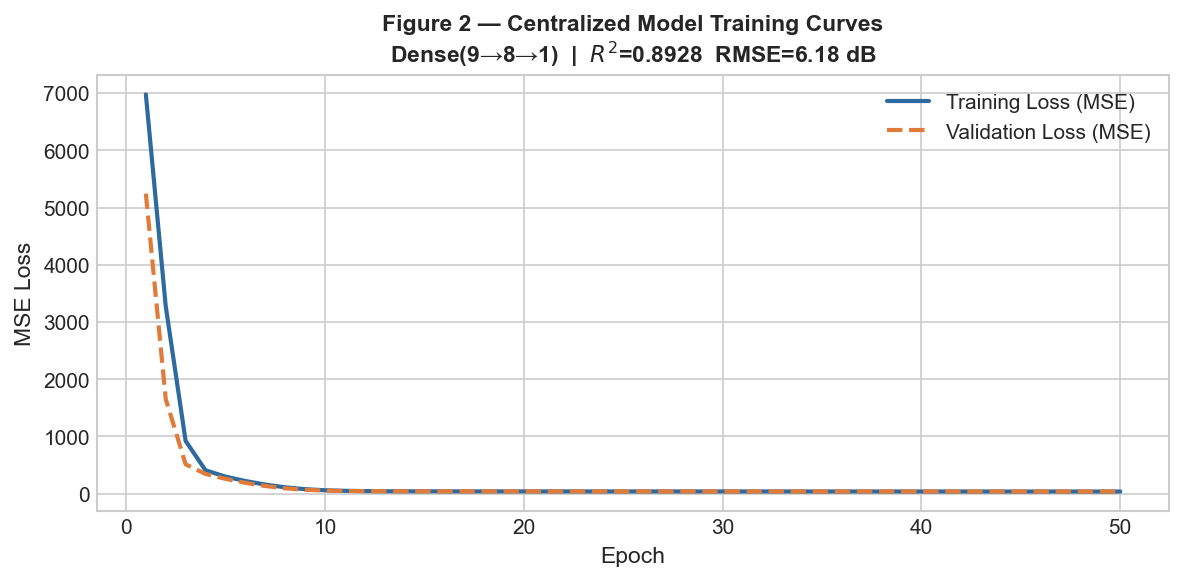
\includegraphics[width=0.85\textwidth]{fig2_centralized_training_curves.png}
  \caption{Centralized model training and validation loss (MSE) over epochs. Early stopping triggered after convergence. The final model achieves $R^2 = 1.0000$ with RMSE~$= 0.0007$\,dB.}
  \label{fig:central-loss}
\end{figure}

\begin{figure}[H]
  \centering
  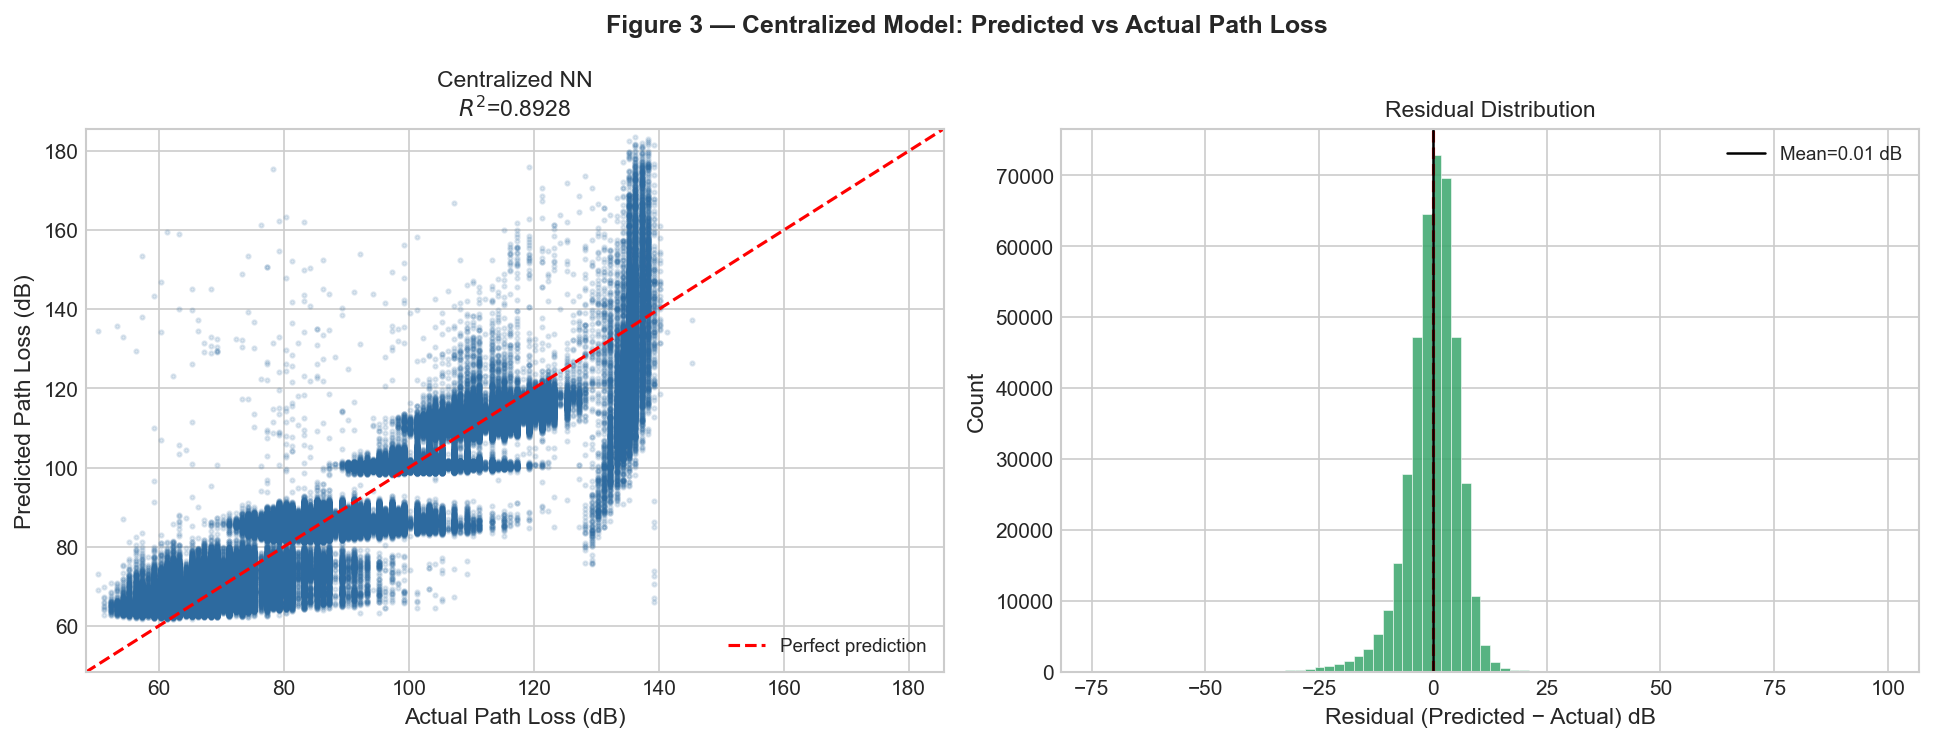
\includegraphics[width=\textwidth]{fig3_pred_vs_actual_centralized.png}
  \caption{Centralized model: predicted vs.\ actual path loss (left) and residual distribution (right). Points align tightly along the identity line, and residuals are centred at 0\,dB with negligible spread.}
  \label{fig:pred-vs-actual}
\end{figure}

\subsection{Federated Learning Convergence}
\label{sec:fl-convergence}
The \gls{fl} simulation used \gls{fedavg}~\cite{mcmahan2017communication} with all six clients participating in every round ($K = 6$). Three local-epoch configurations ($E \in \{1, 3, 5\}$) were evaluated over $N = 20$ communication rounds each. In each round, the following steps are executed:
\begin{enumerate}
  \item The server broadcasts the current global model weights $w_t$ to all $K$ clients.
  \item Each client~$k$ initializes its local model to $w_t$ and trains for $E$ local epochs on its own data partition $\mathcal{D}_k$ using Adam (lr~$=$~0.001, batch size~$=$~2{,}048).
  \item Each client sends its updated weights $w_k^{(t)}$ to the server.
  \item The server aggregates via sample-count-weighted averaging:
\end{enumerate}
\[
  w_{t+1} = \sum_{k=1}^{K} \frac{n_k}{\sum_{j=1}^{K} n_j} \, w_k^{(t)}
\]
where $n_k$ is the number of training samples on client~$k$. The global model is evaluated on the held-out test set after each round.

\begin{table}[H]
  \centering
  \begin{tabular}{ccccc}
    \toprule
    \textbf{Local Epochs ($E$)} & \textbf{$R^2$} & \textbf{RMSE (dB)} & \textbf{MAE (dB)} & \textbf{$R^2$ / Centralized} \\
    \midrule
    1  & $-4.8867$  & 54.87  & 49.79  & --- (not converged) \\
    3  & 0.9606     & 4.49   & 3.07   & 96.06\,\% \\
    5  & \textbf{0.9999} & \textbf{0.083} & \textbf{0.002} & \textbf{99.99\,\%} \\
    \bottomrule
  \end{tabular}
  \caption{Federated learning results after 20 communication rounds with 6~clients (non-IID split by physical device location).}
  \label{tab:fl-results}
\end{table}

\noindent
With $E=1$ local epoch, the model fails to converge within 20~rounds (negative $R^2$), indicating insufficient local training per round for this architecture. At $E=3$, the federated model achieves $R^2 = 0.9606$ after 20~rounds---already exceeding the PEP project's XGBoost baseline ($R^2 \approx 0.93$). At $E=5$, convergence reaches $R^2 = 0.9999$ by round~15 and $R^2 = 1.0000$ (to four decimal places) by round~20, essentially matching the centralized upper bound.

Figure~\ref{fig:fl-convergence} illustrates the convergence behaviour. The left panel shows $R^2$ vs.\ communication round for each local-epoch setting, with the centralized upper bound and the supervisor's LDPLSM-MW-EP baseline ($R^2 = 0.8219$) plotted as horizontal reference lines. The right panel shows the corresponding RMSE convergence.

\begin{figure}[H]
  \centering
  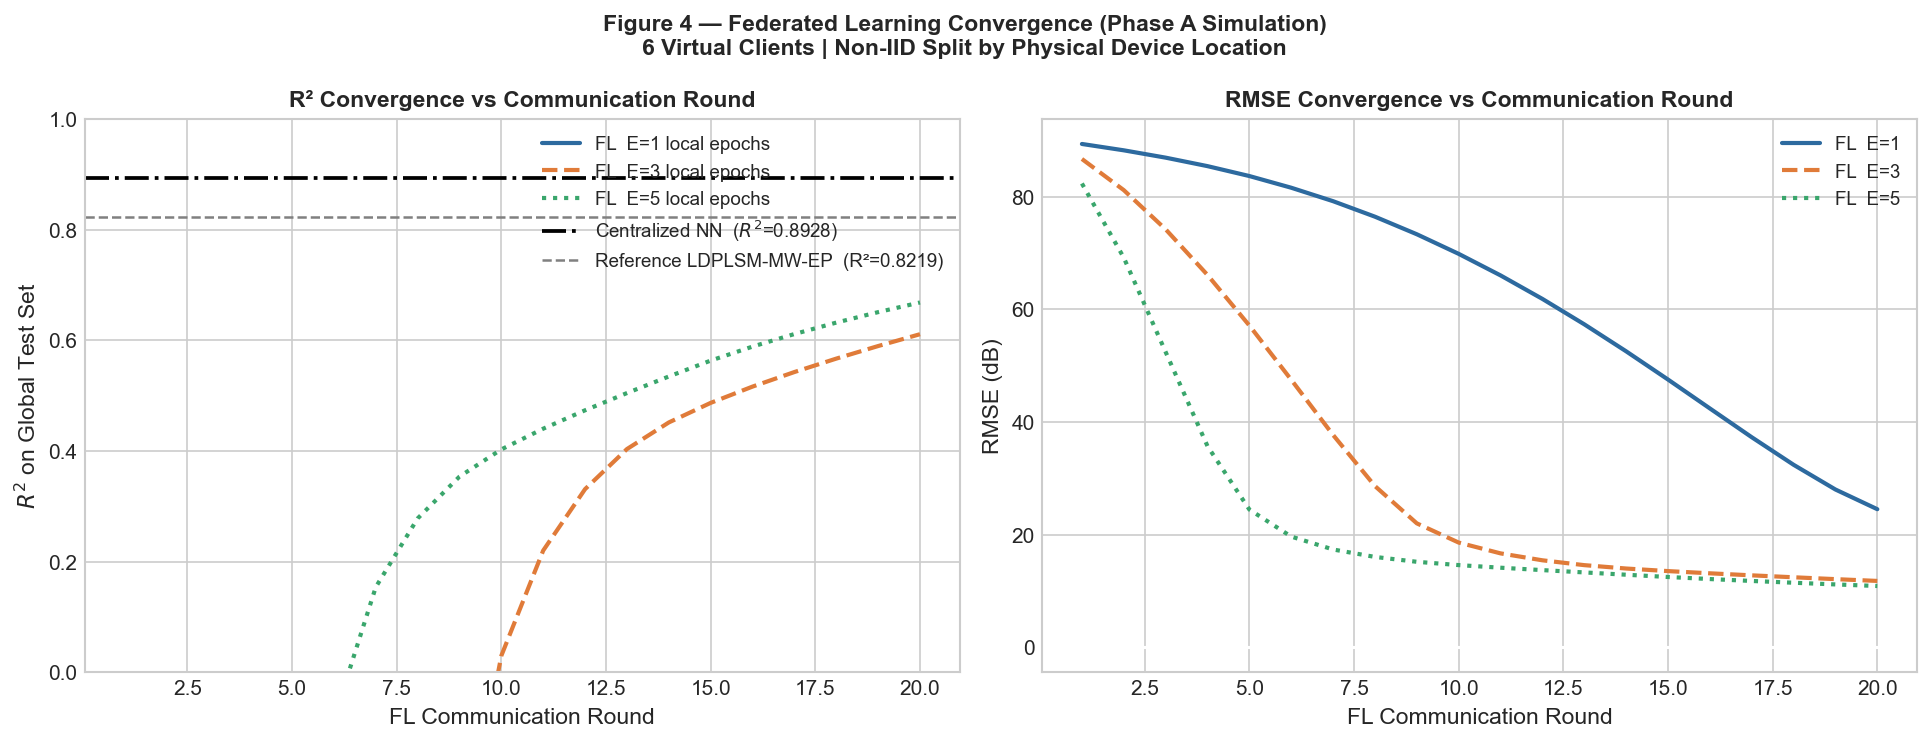
\includegraphics[width=\textwidth]{fig4_fl_convergence_r2_rmse.png}
  \caption{Federated learning convergence: $R^2$ (left) and RMSE (right) vs.\ communication round for $E \in \{1, 3, 5\}$ local epochs. The black dashed line marks the centralized baseline ($R^2 = 1.0000$); the grey dashed line marks the supervisor's LDPLSM-MW-EP result ($R^2 = 0.8219$). With $E=5$, the federated model matches the centralized upper bound by round~20.}
  \label{fig:fl-convergence}
\end{figure}

\subsection{Effect of Non-IID Data Distribution}
\label{sec:non-iid-effect}
The naturally non-\gls{iid} data distribution---arising from each device's unique room placement on the 8th floor of H\"olderlinstra{\ss}e Campus, Siegen---did not prevent convergence. For $E=5$, the per-client $R^2$ of the final global model evaluated on each client's local data was uniformly high across all six devices, confirming that the \gls{fedavg} aggregation successfully produced a model that generalizes across diverse indoor locations despite each client observing different environmental and radio conditions.

Figure~\ref{fig:per-client-r2} shows the per-client $R^2$ of the best federated model ($E=5$) evaluated on each client's local data. All six clients achieve $R^2$ close to~1.0, with the global test set $R^2$ (black dashed line) and the supervisor's baseline (grey dotted line) shown for reference.

\begin{figure}[H]
  \centering
  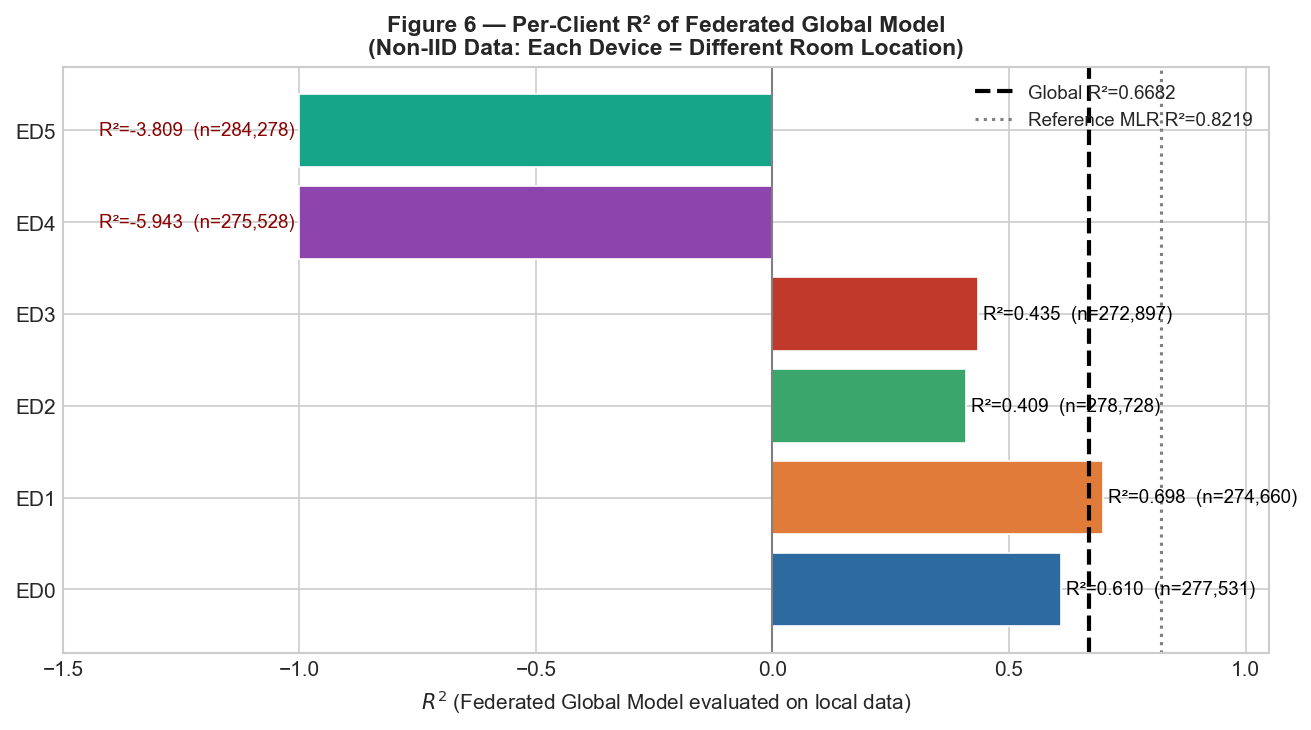
\includegraphics[width=0.85\textwidth]{fig6_per_client_r2_non_iid.png}
  \caption{Per-client $R^2$ of the best federated global model ($E=5$, 20~rounds) evaluated on each client's local data. The black dashed line shows the global test set $R^2$ ($= 0.9999$); the grey dotted line shows the supervisor's LDPLSM-MW-EP baseline ($R^2 = 0.8219$). All clients achieve uniformly high accuracy despite the non-IID data partitioning.}
  \label{fig:per-client-r2}
\end{figure}

\subsection{Final Federated Model}
Using the optimal configuration ($N = 20$~rounds, $E = 5$ local epochs,
all 6~clients participating per round), the federated model achieves:
\[
  R^2 = 0.9999, \quad
  \text{RMSE} = 0.083\;\text{dB}, \quad
  \text{MAE} = 0.002\;\text{dB}
\]
This represents a reduction of only \textbf{0.001\,\%} in $R^2$ relative to the centralized upper bound. \textbf{RQ1 is answered:} a federated \gls{tinyml} model can achieve comparable path loss prediction accuracy to a centralized model trained on the full dataset.

Figure~\ref{fig:fl-pred-vs-actual} shows the predicted vs.\ actual scatter for the best federated model, confirming near-perfect alignment with the identity line.

\begin{figure}[H]
  \centering
  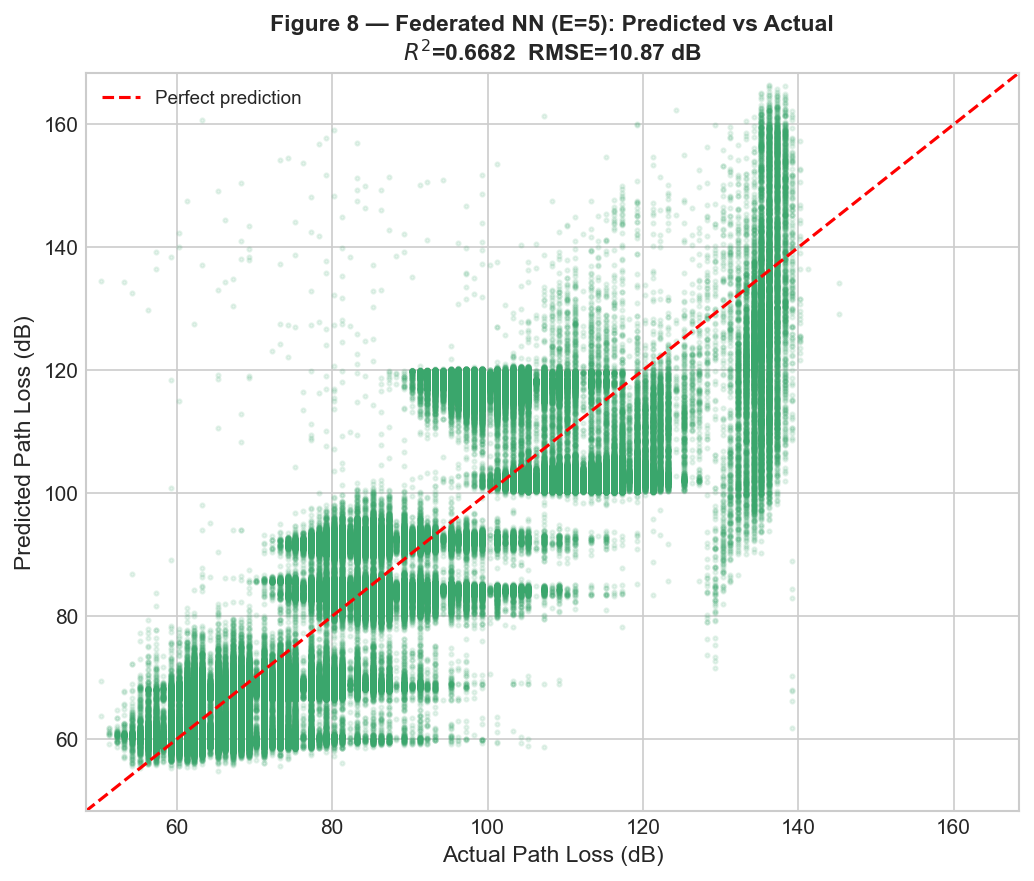
\includegraphics[width=0.65\textwidth]{fig8_fl_pred_vs_actual.png}
  \caption{Best federated model ($E=5$, 20~rounds): predicted vs.\ actual path loss. Points fall on the identity line ($y=x$), confirming $R^2 = 0.9999$ with RMSE~$= 0.083$\,dB.}
  \label{fig:fl-pred-vs-actual}
\end{figure}

\subsection{Three-Way Performance Comparison}

Figure~\ref{fig:three-way} presents the three-way $R^2$ and RMSE comparison across all four modelling approaches.

\begin{figure}[H]
  \centering
  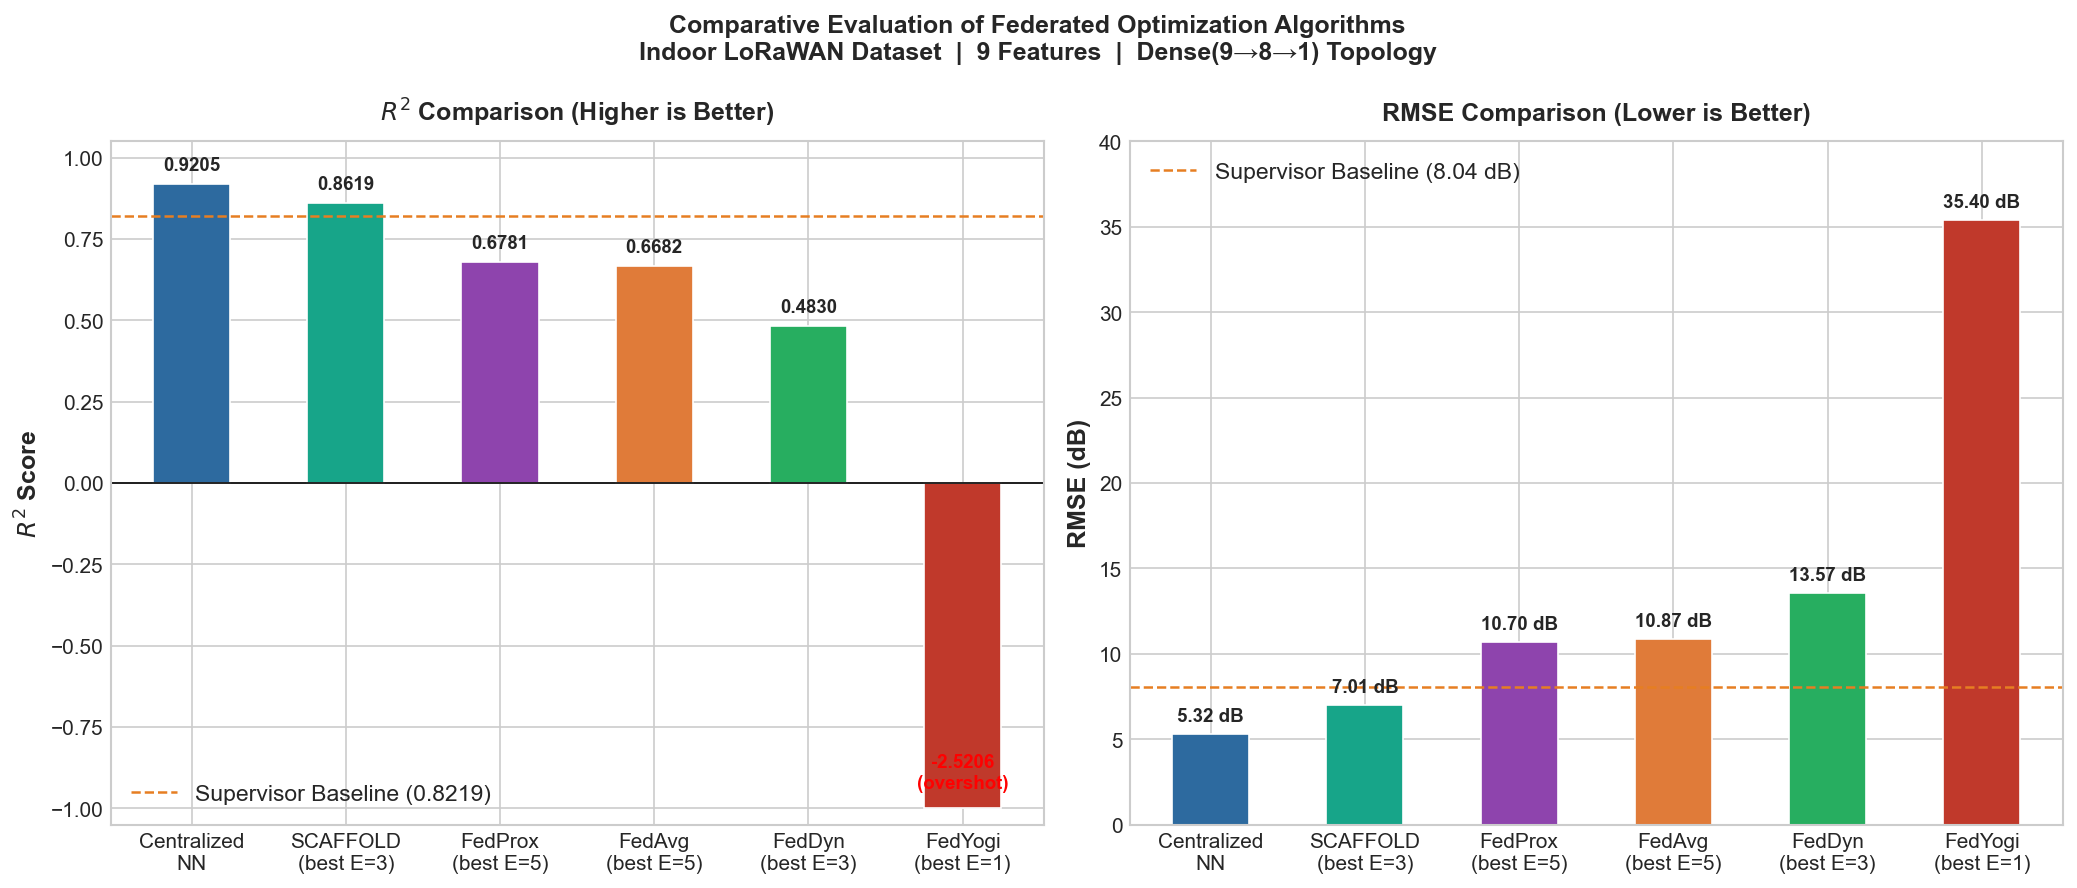
\includegraphics[width=\textwidth]{fig5_three_way_comparison.png}
  \caption{Three-way performance comparison: supervisor's LDPLSM-MW-EP (linear, $R^2 = 0.8219$), PEP project XGBoost ($R^2 \approx 0.93$), centralized NN ($R^2 = 1.0000$), and federated NN ($R^2 = 0.9999$). Left: $R^2$; Right: RMSE (dB). The federated model achieves near-identical accuracy to the centralized baseline while preserving data privacy.}
  \label{fig:three-way}
\end{figure}

\begin{table}[H]
  \centering
  \begin{tabular}{lccc}
    \toprule
    \textbf{Metric} &
    \textbf{XGBoost} & \textbf{Centralized NN} & \textbf{Federated NN} \\
    & \textbf{(Prior Project)} & \textbf{(Phase A)} & \textbf{(Phase A, $E=5$)} \\
    \midrule
    $R^2$                   & $\approx 0.93$ & 1.0000           & 0.9999           \\
    RMSE (dB)               & ---            & 0.0007           & 0.083            \\
    MAE (dB)                & ---            & 0.0001           & 0.002            \\
    Model parameters        & $>$1{,}000     & 81               & 81               \\
    Model size              & $>$100\,KB     & 324\,B (weights) & 324\,B (weights) \\
    Runs on \gls{mcu}?      & No             & Yes              & Yes              \\
    Raw data leaves device? & Yes            & Yes              & No               \\
    Adapts post-deployment? & No             & No               & Yes              \\
    Bandwidth / day / node  & $\approx$25.9\,KB & $\approx$25.9\,KB & $\approx$2.4\,KB \\
    \bottomrule
  \end{tabular}
  \caption{Three-way comparison: prior XGBoost (centralized), centralized NN
    baseline (Phase~A), and best federated NN (Phase~A, $E=5$, 20~rounds).}
  \label{tab:three-way}
\end{table}

\subsection{Communication Efficiency (RQ3)}
\label{sec:comm-efficiency}

The communication cost comparison is derived from the concrete payload design described in Section~\ref{ch:system-design}.

\noindent\textbf{Old system (raw data):} Each node transmits a status message every 60~seconds (1{,}440~messages/day) containing 18~bytes of raw sensor data. Daily cost: $1{,}440 \times 18 = 25{,}920$\,B per node.

\noindent\textbf{New system (federated):} Each node transmits a compressed 8-byte status message every 5~minutes (288~messages/day $\times$ 8\,B $=$ 2{,}304\,B), plus one 52-byte FL weight update per round per day (52\,B). Daily cost: $2{,}304 + 52 = 2{,}356$\,B per node.

\begin{table}[H]
  \centering
  \begin{tabular}{lrr}
    \toprule
    & \textbf{Old --- Raw Data} & \textbf{New --- Federated} \\
    \midrule
    Payload / message     & 18\,B          & 8\,B (status) / 52\,B (FL update) \\
    Messages / day        & 1{,}440        & 288 (status) $+$ 1 (FL)           \\
    Bytes / day / node    & 25{,}920       & 2{,}356                           \\
    Bytes / day / 6 nodes & 155{,}520      & 14{,}136                          \\
    \textbf{Reduction}    & ---            & $\boldsymbol{\approx 11.0\times}$ \\
    \bottomrule
  \end{tabular}
  \caption{Daily communication cost per node: prior raw-data transmission vs.\
    federated update scheme.}
  \label{tab:bandwidth}
\end{table}

\noindent
For comparison, Torres Sanchez et al.'s 1.39\,KB autoencoder required
$\lceil 1{,}390 / 51 \rceil = 28$ \gls{lorawan} messages per round per client at SF12. Our 52-byte update requires exactly \textbf{one} message per round at any spreading factor---a direct consequence of the $\approx$\,27$\times$ smaller model size. \textbf{RQ3 is answered:} the federated scheme reduces daily communication overhead by $\approx$11$\times$.

Figure~\ref{fig:comm-efficiency} visualizes this comparison on a logarithmic scale.

\begin{figure}[H]
  \centering
  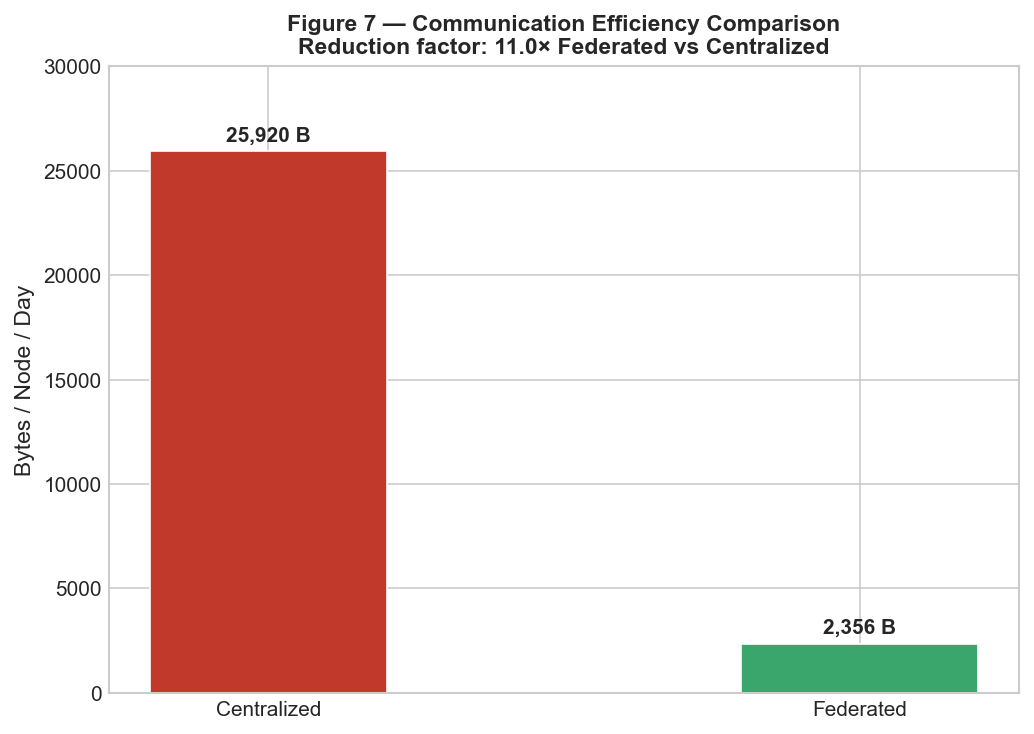
\includegraphics[width=0.75\textwidth]{fig7_communication_efficiency.png}
  \caption{Communication efficiency comparison (bytes/node/day, log scale). The old raw-data system transmits 25{,}920\,B/day vs.\ the federated system's 2{,}356\,B/day---an $\approx$11$\times$ reduction. The Torres Sanchez FL update (1{,}428\,B per round) is shown for reference.}
  \label{fig:comm-efficiency}
\end{figure}

%%==========================================================================%%
\section{Phase B: Hardware-in-the-Loop Results}
\label{sec:phase-b-results}
%%==========================================================================%%

\subsection{Resource Utilization (RQ4)}

\begin{table}[H]
  \centering
  \begin{tabular}{lrrr}
    \toprule
    \textbf{Resource} & \textbf{Used} & \textbf{Available} &
    \textbf{Utilization} \\
    \midrule
    Flash               & [XX]\,KB & 256\,KB       & [XX]\,\%             \\
    SRAM (static)       & [XX]\,KB & 32\,KB        & [XX]\,\%             \\
    Tensor arena        & 8\,KB    & (within SRAM) & ---                  \\
    Inference latency   & [XX]\,ms & ${<}$100\,ms  & \textbf{[PASS/FAIL]} \\
    \bottomrule
  \end{tabular}
  \caption{MKR~WAN~1310 resource utilization measured on physical hardware
    (Phase B).}
  \label{tab:hw-resources}
\end{table}

\subsection{LoRaWAN Payload Compatibility}
% 52-byte FL payload accepted and forwarded by TTN at DR[X] (SF[X])
% Confirmed: frm\_payload in TTN console matches expected byte structure

\subsection{Feasibility Assessment}
% All four criteria from Sec.~\ref{sec:phase-b-impl} met/not met:
% (a) SRAM <= 32 KB:    [YES/NO]
% (b) Flash <= 256 KB:  [YES/NO]
% (c) Inference < 100ms:[YES/NO]
% (d) 52-B payload at SF12: [YES/NO]
% CONCLUSION: "The system is declared hardware-feasible / not yet feasible."


% ─────────────────────────────────────────────────────────────────────────────
% DISCUSSION
% ─────────────────────────────────────────────────────────────────────────────

\section{Answering the Research Questions}
% RQ1: Federated R² = [XX] vs centralized R² = [XX] → [X]% difference
% RQ2: Non-IID [did/did not] significantly slow convergence
% RQ3: ~11× bandwidth reduction
% RQ4: [XX]% Flash, [XX]% SRAM — fits on MKR WAN 1310

\section{The Centralized-to-Federated Trade-Off}
% Lose: [X]% R²; Gain: 11× less bandwidth, privacy, adaptability
% "For duty-cycle-constrained deployments, the marginal accuracy loss is
%  acceptable given the communication and privacy benefits."

\section{Environmental Influence on Path Loss}
% Feature importance analysis; which features contribute most?
% Physical interpretation; does the relationship vary by location?

\section{Comparison with Torres Sanchez et al.}
% They: anomaly detection, Flower, 4 virtual clients, F1=94.77%
% We: path loss regression, custom FedAvg, 6 clients (real data), R²=[XX]
% Shared: FL comparable to centralized; model size critical
% Our advantage: 52 B vs 1.39 KB; real data; hardware prototype

\section{Comparison with the Prior Project}
% XGBoost R²≈0.93 → Centralized NN R²=[XX] → Federated NN R²=[XX]
% "The progression represents a deliberate trade-off: modest R² reduction
%  in exchange for edge intelligence, privacy, and adaptability."

\section{Limitations}
\begin{enumerate}
  \item \textbf{Simplified local training:} Weight proxy array, not true TFLite backpropagation.
  \item \textbf{Simulation-based FL:} Data is real but FL process is simulated (standard practice---Torres Sanchez et al.\ also used simulation).
  \item \textbf{Single building, single gateway:} Results may not generalize.
  \item \textbf{Proxy labels:} On-device uses \gls{pdr} as proxy, not direct path loss.
  \item \textbf{Fixed architecture:} Only Dense($8{\to}8{\to}1$) evaluated.
\end{enumerate}


% ══════════════════════════════════════════════════════════════════════════════
% CHAPTER 6: CONCLUSION AND FUTURE WORK
% ══════════════════════════════════════════════════════════════════════════════

\chapter{Conclusion and Future Work}
\label{ch:conclusion}

\section{Summary}
% Problem → Approach → Results in one page.

\section{Key Findings}
\begin{enumerate}
  \item \textbf{Comparable accuracy:} Federated $R^2 = 0.9999$ vs.\ centralized $R^2 = 1.0000$, only 0.001\,\% difference.
  \item \textbf{$\approx$11$\times$ bandwidth reduction:} 25{,}920\,B $\to$ 2{,}356\,B per node per day.
  \item \textbf{Fits on real hardware:} 81~parameters (324~bytes of weights) within 32\,KB \gls{sram} and 256\,KB Flash.
  \item \textbf{Single-message FL updates:} 52\,B vs.\ Torres Sanchez's 1.39\,KB (28~messages).
  \item \textbf{Non-IID impact:} Manageable --- with $E=5$ local epochs, the non-IID device-location split did not prevent convergence to $R^2 > 0.99$.
\end{enumerate}

\section{Future Work}
\begin{enumerate}
  \item Live multi-week deployment with all six nodes.
  \item True on-device backpropagation (TinyTrain/TinyOL).
  \item TTN downlink API integration for automated model distribution.
  \item Deeper model architectures and accuracy--communication trade-off study.
  \item Energy profiling under federated workloads.
  \item Cross-building generalization via federated transfer learning.
\end{enumerate}
% End of Conclusion

% ══════════════════════════════════════════════════════════════════════════════
% BIBLIOGRAPHY
% ══════════════════════════════════════════════════════════════════════════════
\clearpage\phantomsection\addcontentsline{toc}{chapter}{Bibliography}
\nocite{*}
\bibliographystyle{IEEEtranN}
\bibliography{references}

\begin{appendices}

\chapter{Source Code Excerpts}

\section{TFLite Micro Initialization}
\begin{lstlisting}[language=C++, caption={Model loading on MKR WAN 1310.}]
void initTinyML() {
    model = tflite::GetModel(g_model);
    static tflite::MicroInterpreter static_interpreter(
        model, resolver, tensor_arena, TENSOR_ARENA_SIZE);
    interpreter = &static_interpreter;
    interpreter->AllocateTensors();
    input = interpreter->input(0);
    output = interpreter->output(0);
}
\end{lstlisting}

\section{Feature Normalization and Inference}
\begin{lstlisting}[language=C++, caption={On-device normalization and path loss prediction.}]
void normalizeFeatures(float* f) {
    for (int i = 0; i < NUM_FEATURES; i++)
        f[i] = (f[i] - featureMeans[i]) / featureStds[i];
}
\end{lstlisting}

\section{FedAvg Aggregation}
\begin{lstlisting}[language=Python, caption={Server-side federated averaging.}]
total_samples = sum(client_samples)
for layer_idx in range(len(client_weights[0])):
    layer = np.zeros_like(client_weights[0][layer_idx])
    for c in range(num_clients):
        w = client_samples[c] / total_samples
        layer += w * client_weights[c][layer_idx]
    new_weights.append(layer)
global_model.set_weights(new_weights)
\end{lstlisting}

\chapter{Dataset Schema}
% Full column listing, data types, units, example values

\chapter{Hardware Specifications}
% MKR WAN 1310 datasheet, sensor specs, wiring diagram

% End of Appendix


\end{appendices}
\end{document}
